\section{Probably Approximately Correct (PAC) Learning}
Machines can't compute everything. There are undecidable problems (Turning's halting problem, Post's correspondence problem). \\
Formal logic can't prove everything (G\"{o}del's incompleteness theorem: There are infinitely many truths about arithmetic that cannot be proven formally)
\begin{itemize}
	\item \textbf{Statistical Learning Theory: } Framework for ML aiming at learning \textbf{functions from data}
	\item \textbf{PCA learning: } subfield of ML concerned with the question of \textit{what is learnable and how much can we learn something by empirically minimizing a cost function}.
\end{itemize}

\begin{minipage}{\columnwidth}
\textbf{The learning problem:}
\begin{center}
	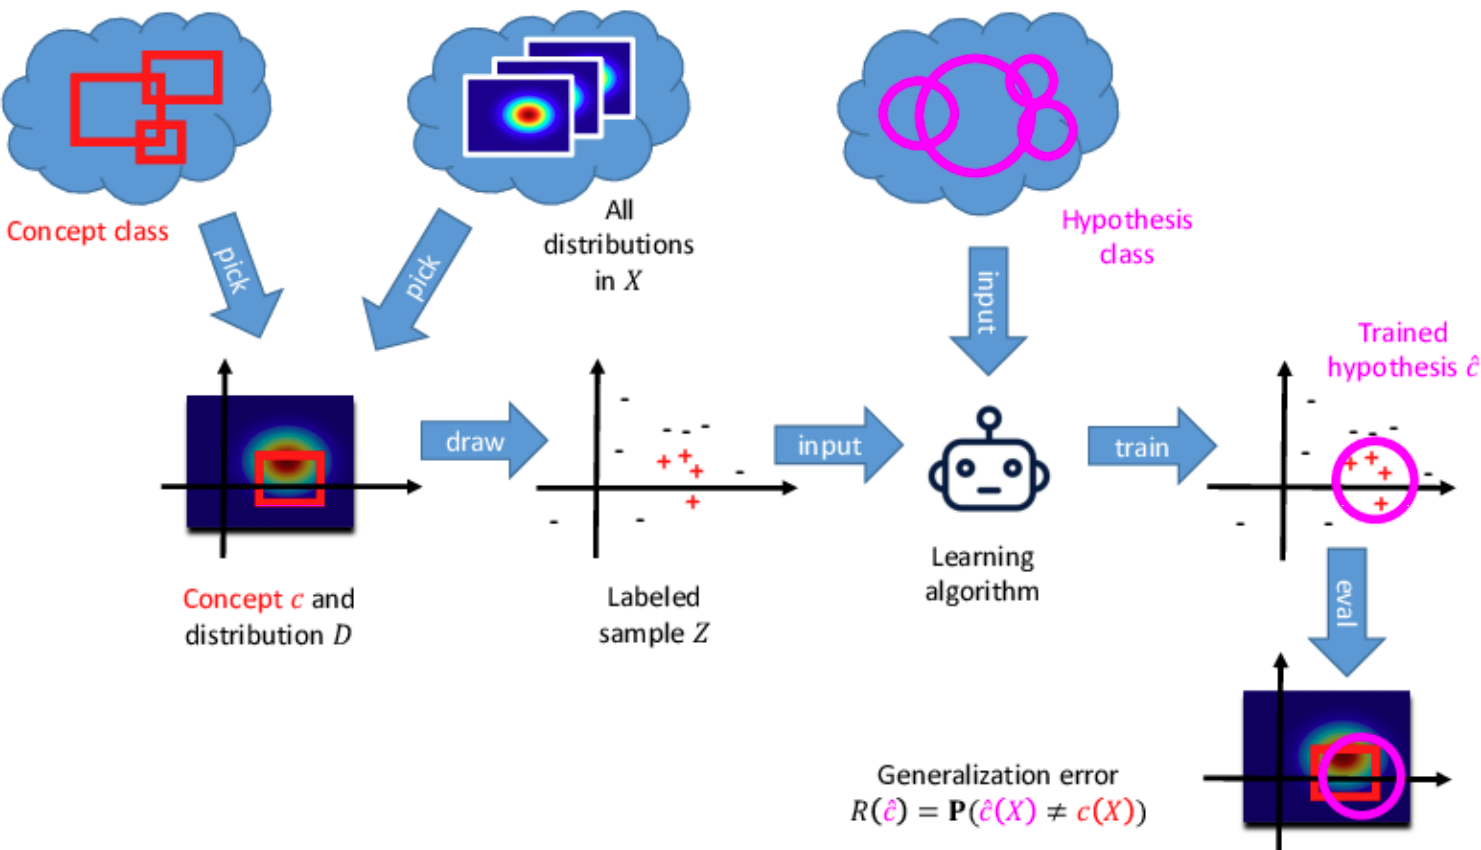
\includegraphics[width=\columnwidth]{images/13-learning-problem}
\end{center}
\end{minipage}
The generalization error measures the distance between the concept $c$ and the trained hypothesis $\hat c$.
\begin{itemize}
	\item The generalization error is not computable by the learner: \\ $\mathcal R(\hat c) := \P(\hat c(X) \neq c(X))$
	\item Empirical error is computable by the learner: \\
	$ \hat{\mathcal R}_n(\hat c) := \sumin \mathbf 1_{\hat c(x_i)\neq c(x_i)}$ \\
	It can be shown that $\E_{X, X_1, ..., X_N}\left[\hat{\mathcal R}_n(\hat c(X))\right] = \mathcal R(\hat c)$
\end{itemize}
\subsection{Notions from statistical learning theory}
\begin{itemize}
	\item \textbf{Instance space $\mathcal X$} Seit of instances or objects in the learner's world
	\item \textbf{Concept: } subset $c$ of $\mathcal X$ (function $c:\mathcal X\to \{0,1\}$ for binary classification).
	\item \textbf{Concept Class: } Set of concepts we wish to learn
	\item \textbf{Hypothesis class: } Other set of concepts that we use to learn a target concept from the concept class.
	\item No additional prior knowledge on $\mathcal X$ is available. This differs from Bayesian approaches.
\end{itemize}



\subsection{The PAC Learning Model}
\begin{itemize}
	\item A concept class $C$ is \textbf{PAC learnable} from a hypothesis class $\mathcal H$ if there is an algorithm that can lern every concept in $\mathcal C$.
	\item If the algorithm runs polynomial time to $1/\epsilon$ and $1/\delta$, we say that $\mathcal C$ is \textbf{efficiently PAC learnable}. ($\epsilon$ error parameter, $\delta$ confidence value)
\end{itemize}






\subsection{Rectangle Learning}
Axis-Aligned rectangles are PAC learnable.
\begin{itemize}
	\item $\mathcal C$ concept of all axis-aligned rectangles. \\
	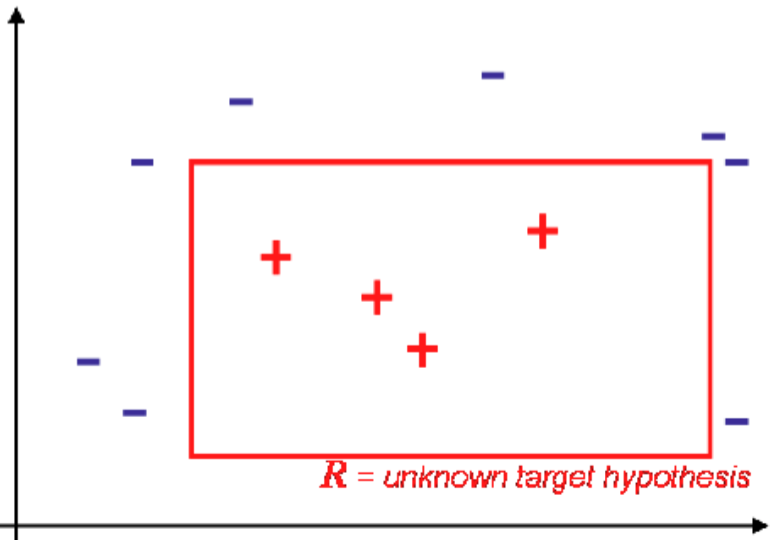
\includegraphics[width = 0.6\columnwidth]{images/13-rectangle-learning}
	\item We show $\mathcal C$ can be learned from $\mathcal H = \mathcal C$
	\item Consider $\mathcal A$ that outputs smalles rectangle $\hat R$ containing all positively labeled points. \textbf{We show that $\mathcal A$ can learn any concept $R\in \mathcal C$
}\end{itemize}

\textbf{How do we prove that $\mathcal A$ learns rectangles?}\\
\begin{itemize}
	\item Define event $\RIG$ \textit{($\hat{\mathcal R}$ is good enough)}, such that
	$$
		\P(\mathcal R(\hat R)\leq \epsilon) \geq \P(\RIG)\geq 1 - 4\exp\left(-\frac{n\epsilon}{4}\right)
	$$
	\item Observe we just need to ensure that $1 - 4\exp\left(-\frac{n\epsilon}{4}\right)\geq 1-\delta$ or equivalently
	$$
		n\geq \frac{4}{\epsilon}\ln\frac{4}{\delta}
	$$
	\item We can ensure this by letting
	$$
		n\geq \underbrace{\frac{4}{\epsilon}\times \frac{4}{\delta}}_{\mathit{poly}(1/\epsilon, 1/\delta, 4)} \geq \frac{4}{\epsilon}\ln\frac{4}{\delta}
	$$
\end{itemize}

\subsubsection*{1. Define event $\RIG$} 
\begin{minipage}{0.5\columnwidth}
	Let $T_{\mathit{upper}}^\epsilon$ be the upper strip sucht that $\P(T_{\mathit{upper}}^\epsilon) = \epsilon/4$, ....\\
	$$
		T^\epsilon = \bigcup_i T_i^\epsilon
	$$
	$\RIG$ is the event in which $\hat R$ intersects all 4 strips
\end{minipage}
\begin{minipage}{0.4\columnwidth}
	\begin{center}
		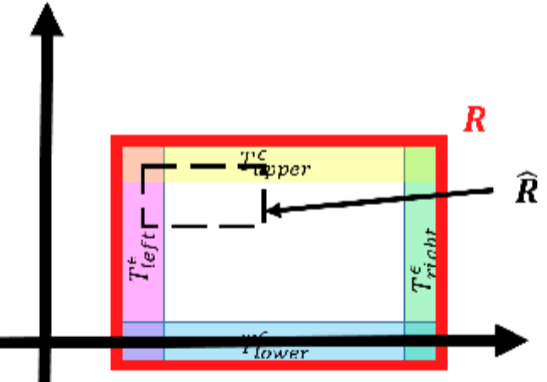
\includegraphics[width=\columnwidth]{images/13-rig}
	\end{center}
\end{minipage}

\subsubsection*{2. Prove $\P(\mathcal R(\hat R)\leq \epsilon) \geq \P(\RIG)\geq 1 - 4\exp\left(-\frac{n\epsilon}{4}\right)$}
\begin{itemize}
	\item Learning algorithm: "tightest fitting rectangle"
	\item Determine
	\begin{align*}
		x_1^{min} = \min\{x_{1,c}:1\leq i\leq n\} \\
		x_1^{max} = \max\{x_{1,c}:1\leq i\leq n\} \\
		x_2^{min} = \min\{x_{2,c}:1\leq i\leq n\} \\
		x_2^{max} = \max\{x_{2,c}:1\leq i\leq n\} \\
	\end{align*}
	\item Select Rectangle $\hat R = \square(x_1^{min}, x_1^{max}, x_2^{min}, x_2^{max})$
\end{itemize}

\textbf{Error: }
\begin{align*}
	\P(\textit{"error"}) 	&= \P(R\Delta\hat R) \\
							&= \P(R - \hat R)\cup (\hat R - R) = \P(R - \hat R)\\
	P(R - \hat R) 			&= \P(\textit{top strip} \cup \textit{bottom s.} \cup \textit{left s.} \cup \textit{right s.}) \\
							&\leq \P(\textit{top}) + \P(\textit{bottom}) + \P(\textit{left}) + \P(\textit{right}) 
\end{align*}

Since the probability to be in one of the strips is $\frac{\epsilon}{4}$ for each strip, we get:
\begin{align*}
	\P(\textit{no sample in top strip)} &= \left(1-\frac{\epsilon}{4}\right)^n \\
	\P(\textit{no sample in any strip)} &\leq 4\left(1-\frac{\epsilon}{4}\right)^n \\
										&\leq 4\exp\left(\frac{n\epsilon}{4} \right)
										&\leq \delta
\end{align*}

Rectangles are PAX learnable, since $n'\geq \frac{4}{\epsilon}\geq \frac{4}{\epsilon}\log\frac{4}{\epsilon}$: 

\begin{align*}
		\P(R\Delta \hat R < \epsilon) &\geq 1 - 4\exp\left(\frac{n\epsilon}{4} \right) \\
		\P(R\Delta \hat R \geq \epsilon) &\leq \underbrace{4}_{\textit{Complexity}}\underbrace{\exp\left(\frac{n\epsilon}{4} \right)}_{\textit{model fit.}} \\
\end{align*}

\subsubsection{Error Prob. for realizable finite hypothesis classes $\mathcal H = \mathcal C$}

$\mathcal C$ finite, $\mathcal H = \mathcal C$, consistent hypothesis $\hat c$ $\forall n< \infty: \hat{\mathcal R}_n(\hat c) = 0$ for any target concept $c\in \mathcal C$, $\hat c\in\argmin_{c\in\mathcal C} \hat R_n(c)$

\begin{align*}
	\P(R(\hat c > \epsilon) &= \P(\max_{c\in\mathcal X:\hat R_n=0} R(x) > \epsilon) \\
							&\leq \sum_{c\in\mathcal C} \P(R(c) > \epsilon\land \hat R_n(c) = 0) \\
							&\leq |\mathcal C|(1-R(c))^n \leq |\mathcal C|e^{n\epsilon} \leq \delta \\
							&\leq |\mathcal C|(1-\epsilon)^n \leq |\mathcal C|e^{n\epsilon} \leq \delta \\
	\implies -n\epsilon + \log|\mathcal C| &\leq \log\delta \\
	\implies n&\geq \frac{1}{\epsilon}\left(\log|\mathcal H| + \log\frac{1}{\delta} \right)
\end{align*}

Further: 
\begin{align*}
	\P(\mathcal R(\hat c)\leq \epsilon) &\geq 1 - \delta &\textit{ bounds the success probability $\delta$}\\
	\P(\mathcal R(\hat c)> \epsilon) &\leq \delta 		&\textit{ bounds the error probability $\epsilon$}
\end{align*}

\begin{highlight}{Proving (efficient) PAC learnability}
\textit{To prove PAC learnability, we have to show that}
$$
	\P(\mathcal R(\hat{c}_n^*) \leq \epsilon) \geq 1 -\delta
$$
\textbf{Efficient PAC learnability: }\\ 
Show the algorithm runs polynomial in $\frac{1}{\delta}$ and $\frac{1}{\epsilon}$
\sepline
\textbf{Example in Exercise 8.3 (Concentric Circles).}
\end{highlight}

\subsubsection{The general stochastic setting}
In general, an instance's label is not determined by the underlying concepts. We model this by distribution $\mathcal D$ on $\mathcal X\times \{0,1\}$. (e.g. two patients with similar features have different reactions on same drug).

\begin{itemize}
	\item Training dataset: $\mathcal Z=\{(x_1, y_1), ..., (x_n, y_n)\}$ from $\mathcal D$.
	\item Goal: Find hypothesis $\hat c\in \mathcal H$ with small generalization error 
	$$
		\mathcal R(\hat c) = \P_{x,y\sim \mathcal D}(\hat c(x)\neq y) = \E_{x,y\sim \mathcal D}\left(\mathbf 1_{\hat c(x)\neq y}\right)
	$$
	\item If the bayes optimimal classifier is not in the hypothesis class $\mathcal C$, then it is \textbf{impossible to attain} $\forall 0 < \epsilon \leq \frac{1}{2}:\mathcal R(\hat c)\leq \epsilon$. Instead, we aim to attain the best solution given in the hypothesis class:
	$$
		R(\hat c) - \inf_{c\in\mathcal C}\mathcal R(c) \leq \epsilon
	$$
\end{itemize}

\subsubsection{The general PAC model}
A learning algorithm $\mathcal A$ can learn a concept class $\mathcal C$ from $\mathcal H$ if given {\color{imp3}sufficiently large sample} as input, outputs a hypothesis that \textbf{{\color{imp}generalizes well} {\color{imp2}with high probability}}

\textbf{Definition: } A learning algorithm $\mathcal A$ can learn a concept class $\mathcal C$ from $\mathcal H$ if there is a {\color{imp3} polynomial function $\mathit{poly}$}, such that
\begin{enumerate}
	\item For any distribution $\mathcal D$ on $\mathcal X\times \{0,1\}$ and
	\item for any {\color{imp}$0<\epsilon<1/2$} and {\color{imp2}$0<\delta<1/2$}
\end{enumerate}
if $\mathcal A$ receives as input {\color{imp3} a sample $\mathcal Z$ of size $n\geq \mathit{poly}(1/\epsilon, 1/\delta, \mathit{dim}(\mathcal X)$}, then $\mathcal A$ outputs $\hat c\in\mathcal H$, sucht that
$$
	{\color{imp2}\P_{\mathcal Z\sim \mathcal D^n}\left({\color{imp}\mathcal R(\hat c) - \inf_{c\in\mathcal C}\mathcal R(c)\leq \epsilon }\right) \geq 1 - \delta}
$$

\begin{highlight}{Proving PAC learnability in the General stoch. setting}
\textit{To prove PAC learnability, we have to show that}
$$
	\P(\mathcal R(\hat{c}_n^*) - \inf_{c\in \mathcal C} \mathcal R(c) \leq \epsilon) \geq 1 - \delta
$$

\sepline
\textbf{Example (ex. 8.2): }
Given: \\
$\P(\mathcal R(\hat{c}_n^*) - \inf_{c\in \mathcal C} \mathcal R(c) > \epsilon) \leq \exp(-\epsilon n)$

\begin{enumerate}
	\item Set $\P(\mathcal R(\hat{c}_n^*) - \inf_{c\in \mathcal C} \mathcal R(c) > \epsilon) \leq \exp(-\epsilon n) {\color{imp}\leq \delta}$
	\item Find $n$ sucht that $\exp(-\epsilon n) \leq \delta$
	\item Observe that for this $n$
	\begin{equation*}
		\begin{gathered}
			1 - \P(\mathcal R(\hat{c}_n^*) - \inf_{c\in \mathcal C} \mathcal R(c) \leq \epsilon) \leq \delta \\
			\P(\mathcal R(\hat{c}_n^*) - \inf_{c\in \mathcal C} \mathcal R(c) \leq \epsilon) \leq 1 -\delta
		\end{gathered}
	\end{equation*}
	\textbf{Hence $\mathcal C$ is PAC learnable from itself.}
\end{enumerate}

\end{highlight}
